\chapter{Réalisation de la Solution}

\section*{Introduction}
Ce chapitre présente la réalisation concrète du pipeline de Data Quality sur le Référentiel Tiers de CIH Bank. Tous les contrôles Soda Core s'effectuent exclusivement sur la \textbf{zone RAW} du Data Lake (base Hive \texttt{raw\_nova\_referentieltiers}), qui constitue la copie exacte et non transformée des tables \texttt{CCM\_*} du système opérant Oracle NOVA (\textbf{\uline{le périmètre complet englobe environ 15 tables Tiers ; dans ce chapitre, les tables \texttt{ccm\_npdescription} et \texttt{ccm\_job} serviront d'exemples illustratifs}}). Nous détaillerons successivement l'environnement technique de développement, l'implémentation du script Soda Core, la création des tables Hive de persistance, l'intégration dans un DAG Airflow indépendant, la mise en place des vues Dremio et la réalisation du dashboard Tableau.

% =========================
\section{Environnement technique de développement}

\subsection{Environnement Hadoop et cluster}

Le développement et les tests ont été réalisés dans l'environnement Hadoop de CIH Bank. L'accès aux tables Hive et aux fichiers HDFS est effectué via les interfaces disponibles dans l'environnement Data Office, en utilisant les comptes de service existants du domaine Tiers.

Les versions exactes des composants utilisés dans l'environnement de production sont les suivantes :

\begin{table}[H]
\centering
\begin{tabular}{|l|l|}
\hline
\rowcolor{gray!20}
\textbf{Composant} & \textbf{Version} \\
\hline
Cloudera Data Platform (CDP) & Private Cloud Base 7.1.7 \\
\hline
Apache Hadoop (HDFS / YARN) & 3.1.1 \\
\hline
Apache Hive & 3.1.3 \\
\hline
Apache Spark & 3.2.0 \\
\hline
Apache Airflow & 2.5.1 \\
\hline
Dremio & Enterprise Edition 2026 \\
\hline
Python & 3.9.13 \\
\hline
Soda Core & soda-core-spark 3.0.45 \\
\hline
Tableau Desktop & Professional Edition 2024.1.2 \\
\hline
\end{tabular}
\caption{Versions des composants de l'environnement technique}
\label{tab:versions_composants}
\end{table}

\subsection{Installation hors-ligne de Soda Core}

La politique stricte de sécurité des systèmes d'information (PSSI) de CIH BANK impose une isolation réseau (air-gap) des serveurs du cluster Big Data, interdisant par conséquent tout accès direct à Internet. L'exécution standard de la commande \texttt{pip install} pour rapatrier les dépendances depuis le registre public PyPI est donc impossible.

L'installation de Soda Core et de son connecteur Spark a donc été réalisée via une procédure d'installation hors-ligne (Offline Wheel Installation) :
\begin{enumerate}
    \item \textbf{Téléchargement des archives (Wheels)} : Sur un poste de travail disposant d'un accès à Internet, les archives des paquets \texttt{soda-core} et \texttt{soda-core-spark} ainsi que l'ensemble de leurs sous-dépendances ont été téléchargées au format \texttt{.whl} dans un dossier dédié.
    \item \textbf{Transfert sécurisé} : Le dossier d'archives a été contrôlé puis transféré de manière sécurisée (SFTP/SCP) vers le nœud Edge (Gateway) du cluster.
    \item \textbf{Installation locale} : Sur le nœud Edge, les paquets ont été déployés dans l'environnement virtuel Python (venv) alloué à l'orchestrateur Airflow à l'aide de la commande \texttt{pip}, en forçant la recherche locale :
\end{enumerate}

\begin{lstlisting}[language=bash]
source /opt/airflow/venv_dq/bin/activate
pip install --no-index --find-links=./soda_wheels soda-core-spark
\end{lstlisting}

Cette méthode garantit la reproductibilité de l'environnement de contrôle tout en respectant scrupuleusement les contraintes de sécurité bancaires.

% =========================
\section{Implémentation du moteur DQ — Soda Core}

\subsection{Structure des fichiers du projet DQ}

Le projet DQ est organisé selon l'arborescence suivante :

\begin{lstlisting}
dq_tiers/
|-- dq_tiers_checks.py          # Script principal Python
|-- checks/
|   |-- checks_tiers.yml        # Regles DQ fonctionnelles Tiers
|   |-- checks_csp.yml          # Regles DQ colonnes CSP
|   +-- checks_pipeline.yml     # Regles fraicheur & pipeline
+-- utils/
    +-- hive_writer.py          # Module d'ecriture resultats dans Hive
\end{lstlisting}

\subsection{Fichier de configuration YAML — Règles Métier (\texttt{checks\_tiers.yml})}

\begin{lstlisting}[language=YAML]
# checks_tiers.yml
# Regles Data Quality - Domaine Tiers
# Source : raw_nova_referentieltiers.ccm_npdescription (zone RAW)
# Zone RAW = copie exacte d'Oracle NOVA, aucune transformation appliquee

checks for ccm_npdescription:

  # --- Completude ---
  - missing_count(name) = 0:
      name: "KYC-01 | Completude | Nom"
      fail: error
      attributes:
        criticite: CRITIQUE
        domaine: KYC
        dimension: completeness

  - missing_count(first_name) = 0:
      name: "KYC-02 | Completude | Prenom"
      fail: error
      attributes:
        criticite: CRITIQUE
        domaine: KYC
        dimension: completeness

  - missing_count(birthdate) = 0:
      name: "KYC-03 | Completude | Date de naissance"
      fail: error
      attributes:
        criticite: CRITIQUE
        domaine: KYC
        dimension: completeness

  - missing_count(nationality_country) = 0:
      name: "KYC-04 | Completude | Nationalite"
      fail: warn
      attributes:
        criticite: HAUTE
        domaine: KYC
        dimension: completeness

  # --- Validite ---
  - invalid_count(civility) = 0:
      valid values: ["M.", "MME", "MLLE"]
      name: "KYC-05 | Validite | Civilite hors referentiel"
      fail: warn
      attributes:
        criticite: HAUTE
        domaine: KYC
        dimension: validity

  - invalid_count(gender) = 0:
      valid values: ["M", "F"]
      name: "KYC-06 | Validite | Genre hors referentiel"
      fail: warn
      attributes:
        criticite: HAUTE
        domaine: KYC
        dimension: validity

  # --- Fraicheur ---
  - freshness(batch_datetime_eaac4) < 26h:
      name: "KYC-07 | Fraicheur | Retard batch"
      fail: error
      attributes:
        criticite: HAUTE
        domaine: PIPELINE
        dimension: freshness
\end{lstlisting}



\subsection{Script Python principal (\texttt{dq\_tiers\_checks.py})}

\begin{lstlisting}[language=Python]
# dq_tiers_checks.py
# Pipeline de Data Quality - Referentiel Tiers PP Clients - Zone RAW
# CIH Bank - Data Office
# Auteur : Saad BENDAHOU
# Declenchement : Nouveau DAG Indépendant (00h00)

import argparse
import datetime
from datetime import date
from pyspark.sql import SparkSession
from soda.scan import Scan

def run_dq_checks(run_date: str):
    """
    Execute les controles DQ Soda Core sur les tables Hive
    du domaine Tiers et persiste les resultats.
    """
    # --- 1. Initialisation de la SparkSession ---
    spark = SparkSession.builder \
        .appName("DQ_Tiers_Checks") \
        .enableHiveSupport() \
        .getOrCreate()

    # --- 2. Initialisation du scan Soda Core ---
    scan = Scan()
    scan.set_data_source_name("hive_raw")
    scan.add_spark_session(spark, "hive_raw")

    # --- 3. Chargement des fichiers de regles YAML ---
    scan.add_sodacl_yaml_file("checks/checks_kyc.yml")
    scan.add_sodacl_yaml_file("checks/checks_csp.yml")
    scan.add_sodacl_yaml_file("checks/checks_pipeline.yml")

    # --- 4. Execution des checks ---
    scan.execute()

    # --- 5. Collecte et persistance des resultats de faits ---
    run_timestamp = datetime.datetime.now()
    results_data = []

    for check in scan.get_checks_self():
        passed = check.outcome == "pass"
        score = 100.0 if passed else (50.0 if check.outcome == "warn" else 0.0)
        
        # Recupere le total des lignes et le nombre d'anomalies
        total_rows = spark.table(f"raw_nova_referentieltiers.{check.dataset_name}").count()
        invalid_rows = int(check.check_value or 0) if not passed else 0
        valid_rows = total_rows - invalid_rows
        percentage = (valid_rows / total_rows) * 100.0 if total_rows > 0 else 100.0

        results_data.append((
            run_timestamp,
            "dailyow22",
            check.dataset_name,
            check.column_name or "TRANSVERSE",
            check.name,
            check.attributes.get('dimension', 'completeness'),
            check.attributes.get('criticite', 'HAUTE'),
            check.attributes.get('domaine', 'Tiers'),
            total_rows,
            valid_rows,
            invalid_rows,
            percentage,
            check.outcome,
            score,
            run_date
        ))

    if results_data:
        df = spark.createDataFrame(results_data, [
            "run_timestamp", "dag_name", "table_name", "column_name", "check_name",
            "dimension", "criticite", "domaine", "total_rows", "valid_rows",
            "invalid_rows", "percentage", "state", "score_dq", "run_date"
        ])
        df.write.mode("append").partitionBy("run_date").saveAsTable("dq_results.dq_tiers_results_fact")

    spark.stop()
    print(f"[DQ Tiers] Controles termines pour la date {run_date}")

if __name__ == "__main__":
    parser = argparse.ArgumentParser()
    parser.add_argument("--run_date", type=str, default=str(date.today()))
    args = parser.parse_args()
    run_dq_checks(args.run_date)
\end{lstlisting}

% =========================
\section{Création des tables Hive de persistance}

Les tables de persistance DQ sont créées dans la base Hive \texttt{dq\_results}. Le script HiveQL de création est le suivant :

\begin{lstlisting}[language=SQL]
-- Creation de la base dediee DQ
CREATE DATABASE IF NOT EXISTS dq_results
COMMENT 'Base de resultats Data Quality - CIH Bank Data Office';

-- Table de faits unique pour la Data Quality
CREATE TABLE IF NOT EXISTS dq_results.dq_tiers_results_fact (
    run_timestamp   TIMESTAMP,
    dag_name        STRING,
    table_name      STRING,
    column_name     STRING,
    check_name      STRING,
    dimension       STRING,
    criticite       STRING,
    domaine         STRING,
    total_rows      BIGINT,
    valid_rows      BIGINT,
    invalid_rows    BIGINT,
    percentage      DOUBLE,
    state           STRING,
    score_dq        DOUBLE
)
PARTITIONED BY (run_date DATE)
STORED AS ORC
TBLPROPERTIES ('orc.compress'='SNAPPY');
\end{lstlisting}

% =========================
\section{Création du DAG Airflow indépendant \texttt{daily\allowbreak\_dq\allowbreak\_00}}

\subsection{Ajout de la tâche DQ}

Un nouveau DAG nommé \texttt{daily\allowbreak\_dq\allowbreak\_00} a été créé pour automatiser les contrôles de qualité de façon totalement indépendante de l'ingestion. Placé à 00h00, ce DAG exploite l'orchestrateur pour déclencher le pipeline Python Soda Core, garantissant une exécution modulaire et isolée du moteur de qualité sur le nœud Edge.

\begin{lstlisting}[language=Python]
# DAG indépendant daily_dq_00 (Airflow)
from airflow.operators.python import PythonOperator
from airflow.utils.trigger_rule import TriggerRule
import subprocess

def run_dq_tiers(**context):
    run_date = context['ds']  # Format YYYY-MM-DD
    result = subprocess.run(
        [
            'python',
            '/opt/airflow/scripts/dq/dq_tiers_checks.py',
            '--run_date', run_date
        ],
        capture_output=True,
        text=True
    )
    if result.returncode != 0:
        raise Exception(f"DQ Tiers failed:\n{result.stderr}")

dq_tiers_task = PythonOperator(
    task_id='run_dq_tiers_checks',
    python_callable=run_dq_tiers,
    trigger_rule=TriggerRule.ALL_DONE,
    dag=dag
)

# Positionnement dans le graphe : apres toutes les ingestions CCM_*
[ccm_party_task, ccm_npdescription_task, ccm_job_task,
 ccm_portfolio_task, ccm_context_task] >> dq_tiers_task
\end{lstlisting}

\subsection{Planification et monitoring}

Ce nouveau DAG \texttt{daily\allowbreak\_dq\allowbreak\_00} s'exécute quotidiennement à \textbf{00h00}, deux heures après l'ingestion. La tâche \texttt{BashOperator} déclenche l'exécution du job PySpark de validation de données. Les logs Airflow permettent de suivre l'exécution et de détecter toute anomalie dans le pipeline DQ.

% =========================
\section{Exposition et virtualisation sous Dremio}

Pour exposer les indicateurs de qualité stockés dans Hive vers l'outil BI Tableau sans déplacement physique de données, nous utilisons Dremio en tant que couche de virtualisation de données dans un schéma dédié. Dremio se connecte directement au catalogue Hive Metastore et effectue une jointure sur les clés \texttt{run\_id} et \texttt{query\_id} des trois tables physiques générées par Soda Core.

Le résultat est exposé sous forme d'un unique dataset virtuel nommé \texttt{fact\allowbreak\_tiers\allowbreak\_dq\allowbreak\_consolidated} de 21 colonnes. Dremio sert ainsi de passerelle d'exposition performante grâce à ses accélérations matérielles (réflexions de données). La figure \ref{fig:screenshot_dremio} montre le lignage réel des données au sein de la plateforme Dremio.

\begin{figure}[H]
    \centering
    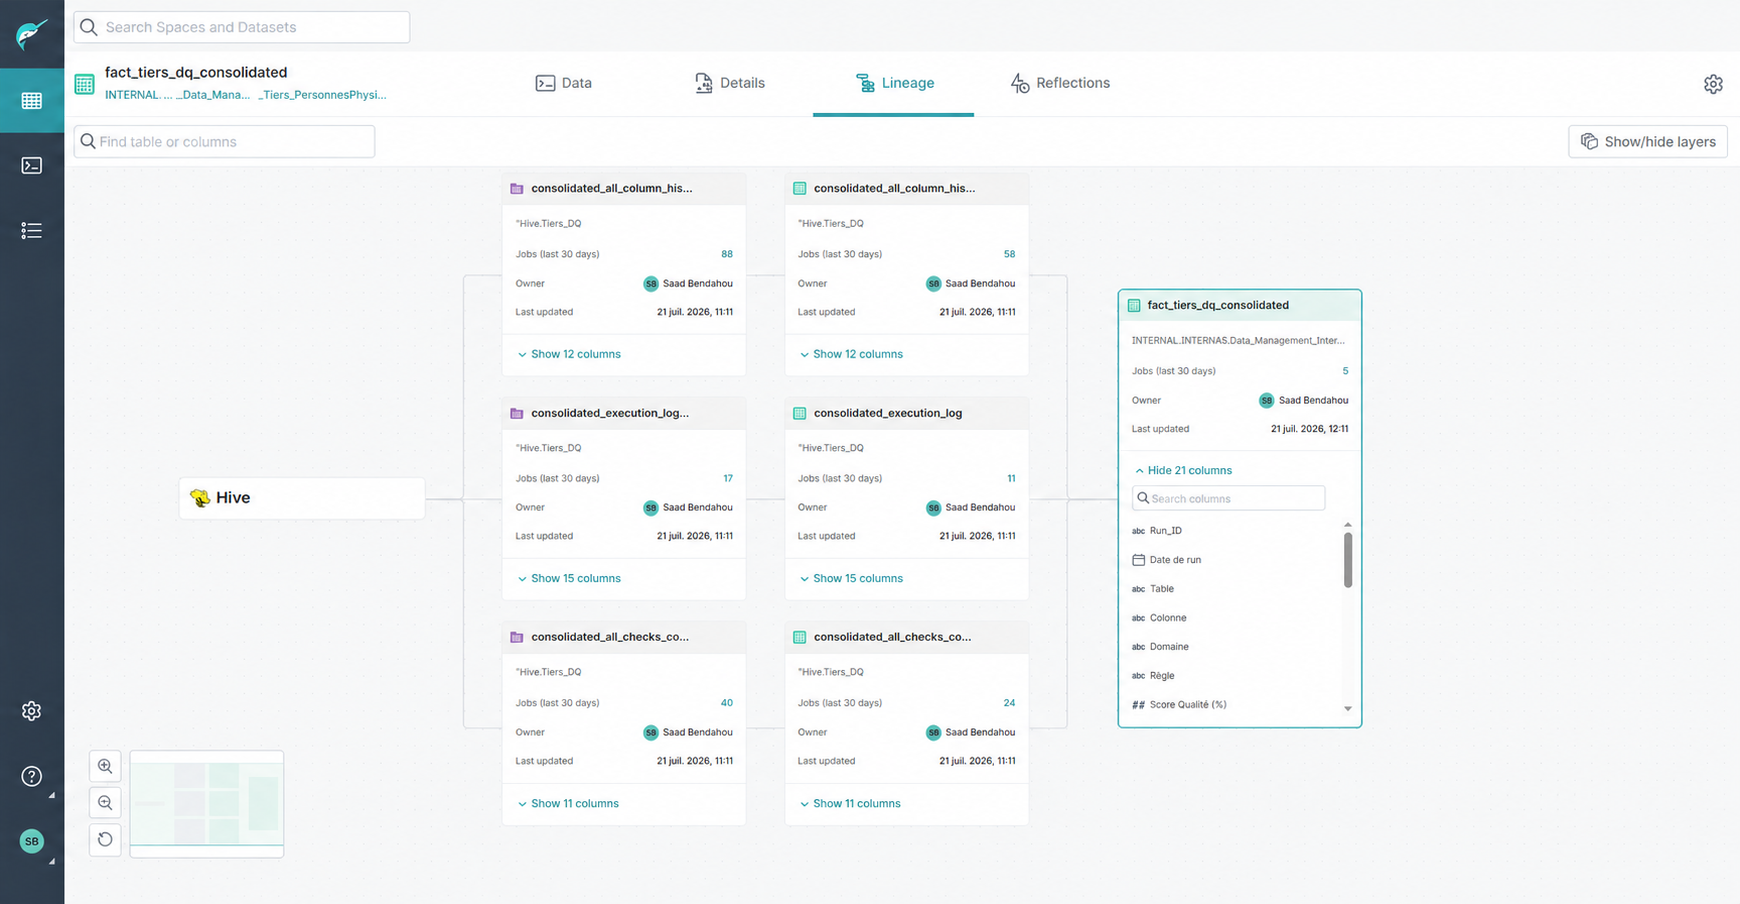
\includegraphics[width=\textwidth, keepaspectratio]{figures/lignage_dremio.png}
    \caption{Lignage des données dans Dremio montrant la création de la vue sémantique \texttt{fact\allowbreak\_tiers\allowbreak\_dq\allowbreak\_consolidated}}
    \label{fig:screenshot_dremio}
\end{figure}

Afin d'optimiser les performances de requêtage, aucune pré-agrégation lourde n'est appliquée au niveau de Dremio. L'exposition de cette grande table de faits consolidée permet de déléguer toute l'intelligence de calcul et de restitution dynamique à l'outil BI Tableau Desktop.

% =========================
\section{Réalisation du dashboard Tableau}

\subsection{Connexion Tableau à Dremio et traitement analytique}

Le dashboard Tableau est connecté à Dremio via le connecteur ODBC/JDBC natif. L'unique vue virtuelle \texttt{fact\allowbreak\_tiers\allowbreak\_dq\allowbreak\_consolidated} est importée comme source de données unique dans Tableau Desktop. 

Tous les filtres (par date d'exécution, par sous-domaine, par dimension de qualité), ainsi que toutes les agrégations (comptage de règles, calculs des moyennes de taux de conformité quotidiens ou scores moyens) sont réalisés de manière dynamique au sein des feuilles de calcul (sheets) et des tableaux de bord de Tableau en tirant directement les champs de la table de faits.


\emph{Note de confidentialité : Il est important de souligner que, pour des raisons évidentes de sécurité et de respect du secret bancaire, les noms de tables réels et certaines données sensibles présentées dans les captures d'écran suivantes ont fait l'objet d'un masquage ou d'un floutage systématique.}

\subsection{Onglet 1 — Vue d'ensemble (Dashboard Global)}

La figure \ref{fig:vuehome} présente la page d'accueil du dashboard, offrant une vision synthétique de l'état de santé du référentiel.

\begin{figure}[H]
    \centering
    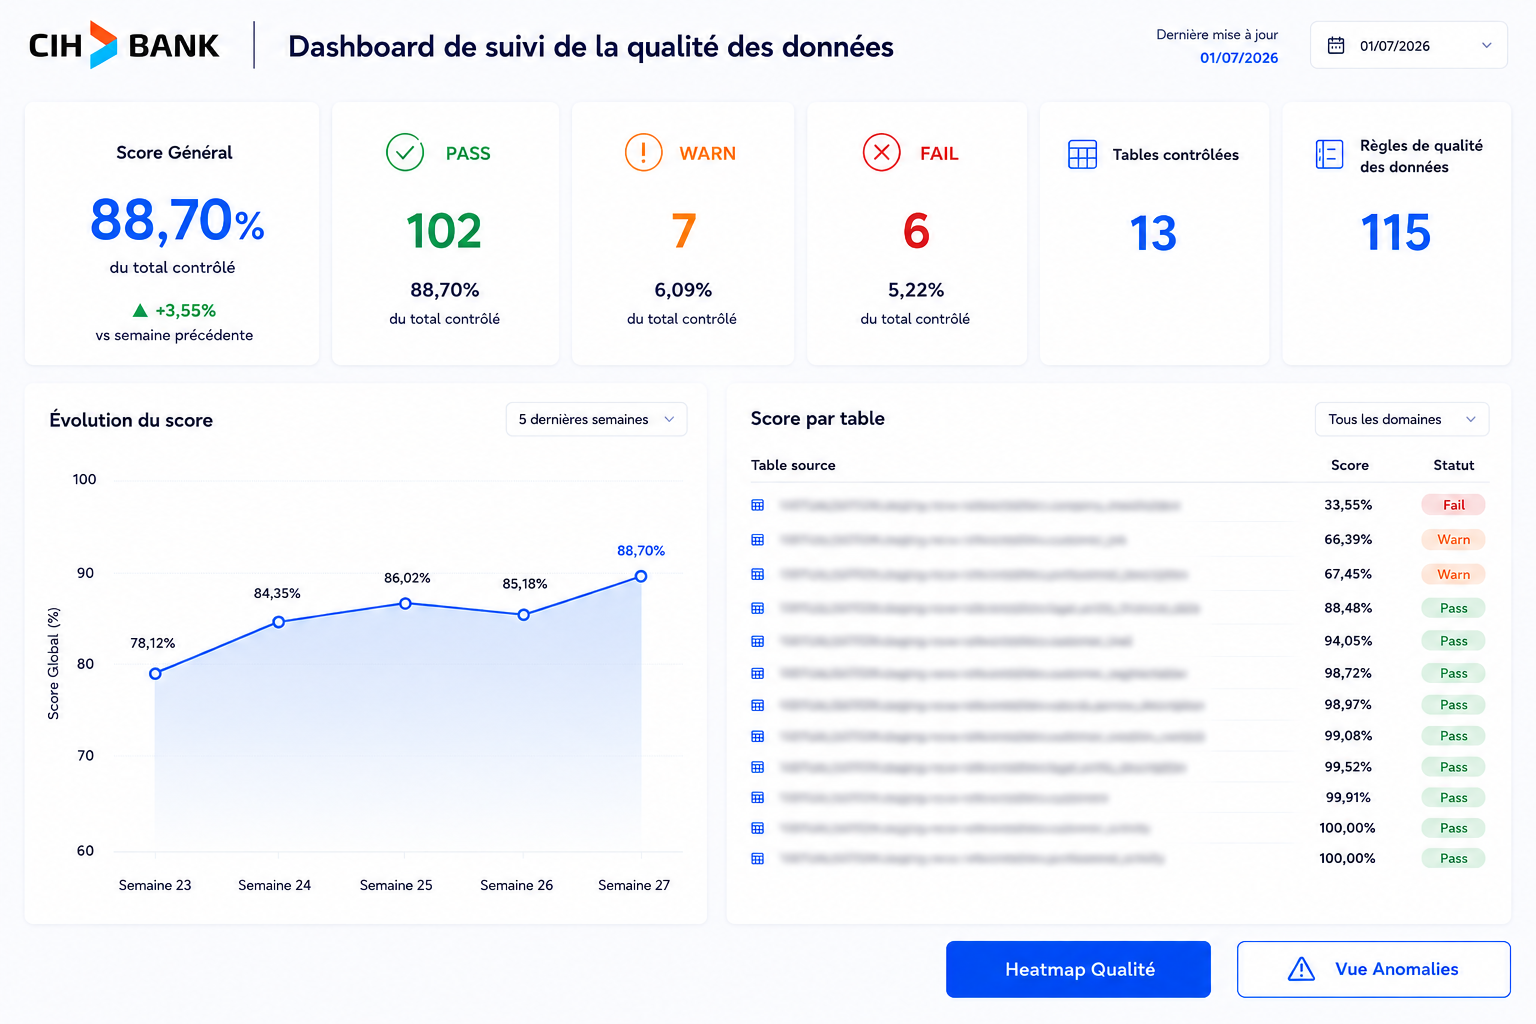
\includegraphics[width=\textwidth]{figures/vuehome.png}
    \caption{Dashboard Tableau — Vue d'ensemble de la qualité des données}
    \label{fig:vuehome}
\end{figure}

Cet onglet centralise les indicateurs de haut niveau :
\begin{itemize}
    \item Le \textbf{Score Général} de qualité (ex: 88,70\%) et sa variation par rapport à la semaine précédente.
    \item La répartition des contrôles par statut : le nombre de tests en succès (PASS), en avertissement (WARN) ou en échec (FAIL), accompagnés de leurs pourcentages respectifs.
    \item Le périmètre évalué (nombre de tables contrôlées et nombre de règles déployées).
    \item L'\textbf{Évolution du score} sur les 5 dernières semaines sous forme de graphique linéaire, permettant d'observer la tendance globale de la qualité.
    \item Un tableau de classement détaillant le \textbf{Score par table}, permettant d'identifier d'un coup d'œil les tables les plus problématiques (marquées en rouge "Fail").
\end{itemize}

\subsection{Onglet 2 — Heatmap Qualité}

La figure \ref{fig:heatmap} présente la vue matricielle détaillée.

\begin{figure}[H]
    \centering
    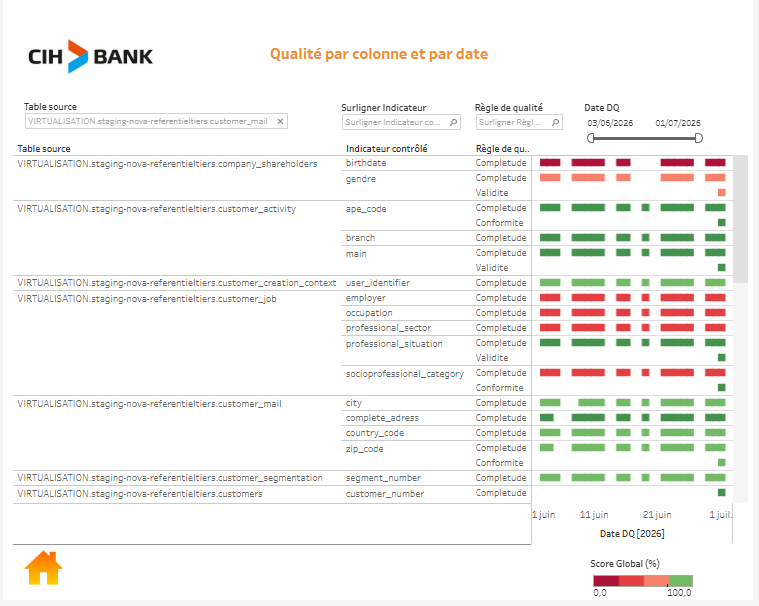
\includegraphics[width=\textwidth]{figures/HEATMAP.png}
    \caption{Dashboard Tableau — Heatmap Qualité par colonne et par date}
    \label{fig:heatmap}
\end{figure}

Cet onglet permet une analyse granulaire du niveau de qualité :
\begin{itemize}
    \item Il liste précisément chaque \textbf{Indicateur contrôlé} (ex: \texttt{birthdate}, \texttt{gender}, \texttt{city}, etc.) associé à sa \textbf{Règle de qualité} (Complétude, Validité, Conformité).
    \item Une \textbf{carte de chaleur (Heatmap) temporelle} colore les résultats par date de scan, allant du rouge (échec total) au vert (succès total). Cette visualisation est extrêmement pertinente pour repérer rapidement des dégradations soudaines (incident de pipeline) ou confirmer l'efficacité d'une campagne de remédiation des données au fil du temps.
\end{itemize}

\subsection{Onglet 3 — Top Anomalies}

La figure \ref{fig:anomaly} présente la vue orientée sur l'analyse et la remédiation.

\begin{figure}[H]
    \centering
    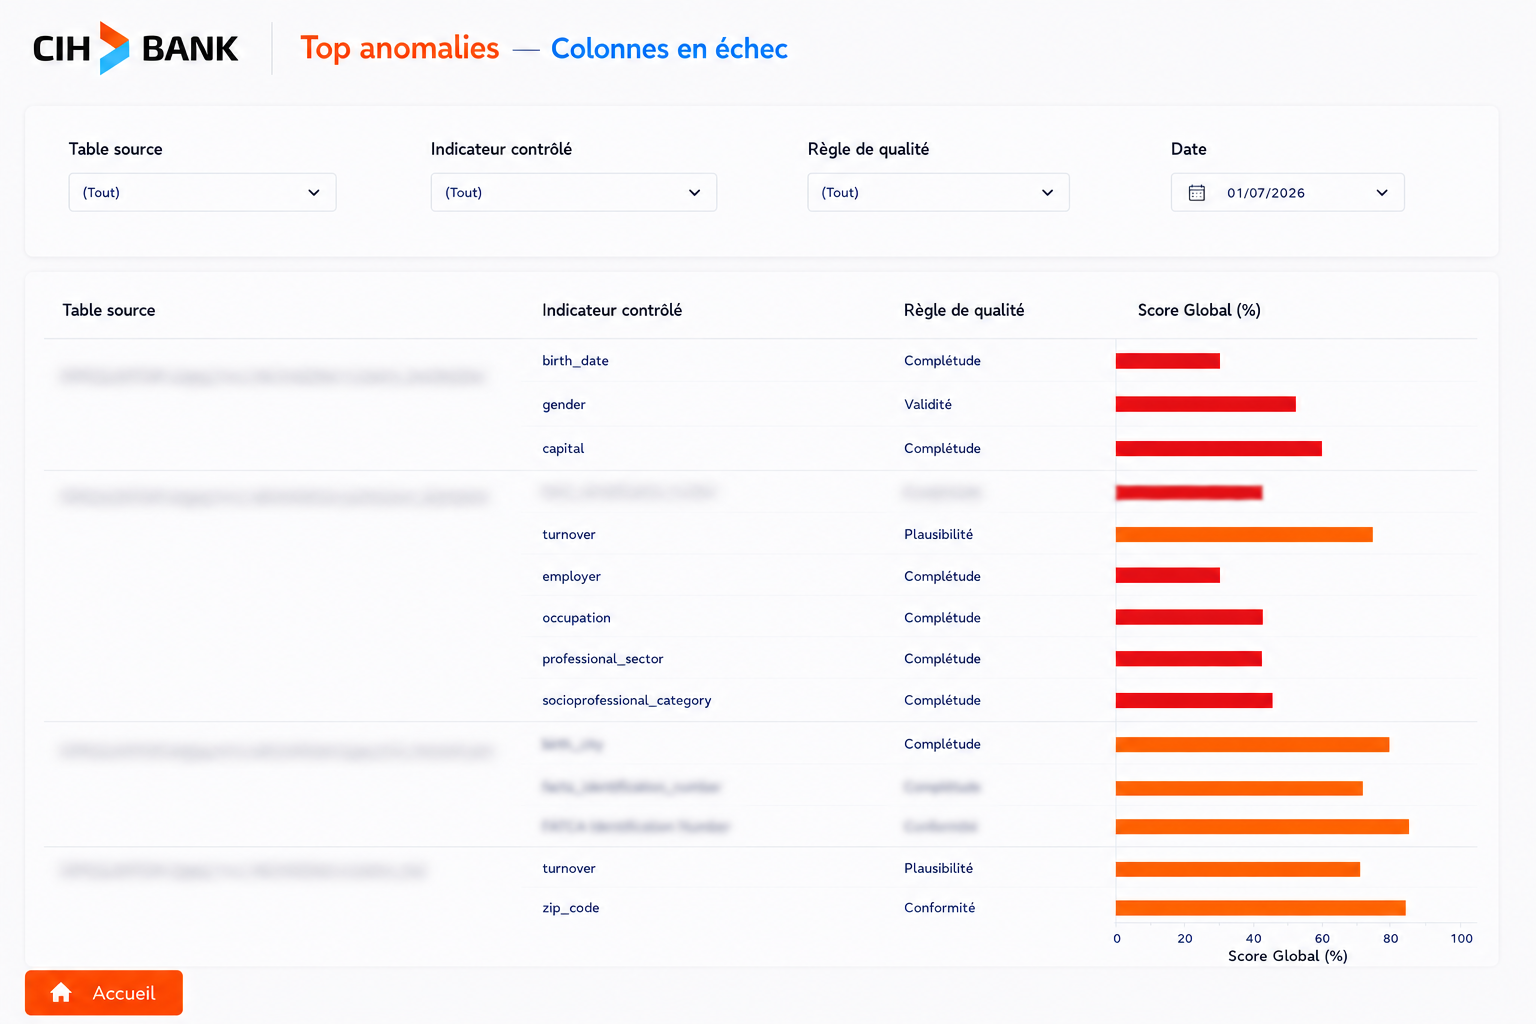
\includegraphics[width=\textwidth]{figures/anomaly.png}
    \caption{Dashboard Tableau — Top anomalies et colonnes en échec}
    \label{fig:anomaly}
\end{figure}

Ce dernier onglet est un véritable outil d'action pour les Data Stewards :
\begin{itemize}
    \item Il cible exclusivement les règles de qualité et les colonnes présentant des taux d'anomalies élevés.
    \item Un diagramme en barres horizontales présente le \textbf{Score Global (\%)} pour chaque indicateur en souffrance. Plus la barre s'approche du rouge et de 0, plus la volumétrie de données non-conformes est critique.
    \item Grâce aux filtres dynamiques situés en haut (par table, par indicateur, par règle ou par date), les utilisateurs métiers peuvent isoler instantanément les axes nécessitant des actions de correction collectives dans l'application source NOVA.
\end{itemize}

\section*{Conclusion}

Ce chapitre a présenté l'implémentation concrète des différents composants du pipeline de Data Quality Tiers : le script Soda Core avec ses fichiers de configuration YAML, les tables Hive de persistance, la tâche Airflow post-ingestion, l'exposition sémantique de Dremio et le dashboard Tableau de visualisation. L'ensemble de ces composants forme un pipeline automatisé, opérationnel chaque nuit à 22h, qui permet de mesurer, historiser et restituer la qualité des données métier du Référentiel Tiers. Le chapitre suivant présente les résultats obtenus lors des premières exécutions.
